% !TEX encoding = UTF-8 Unicode
\documentclass[a4paper, 11pt]{article}
\usepackage[utf8]{inputenc}
\usepackage[T1]{fontenc}
\usepackage[francais]{babel}
\usepackage{fullpage}
\usepackage{hyperref}
\usepackage{graphicx}
\usepackage[nonumberlist]{glossaries}
\usepackage{amssymb,amsmath}
\makeglossaries

\title{{INFO-H-303 : Base de données} \\ Projet - Remise de la première partie}
\author{Thomas \textsc{Herman} \\ Jérôme \textsc{Hellinckx}}


\begin{document}
\maketitle

\section*{Modèle entité-association}
\begin{center}
	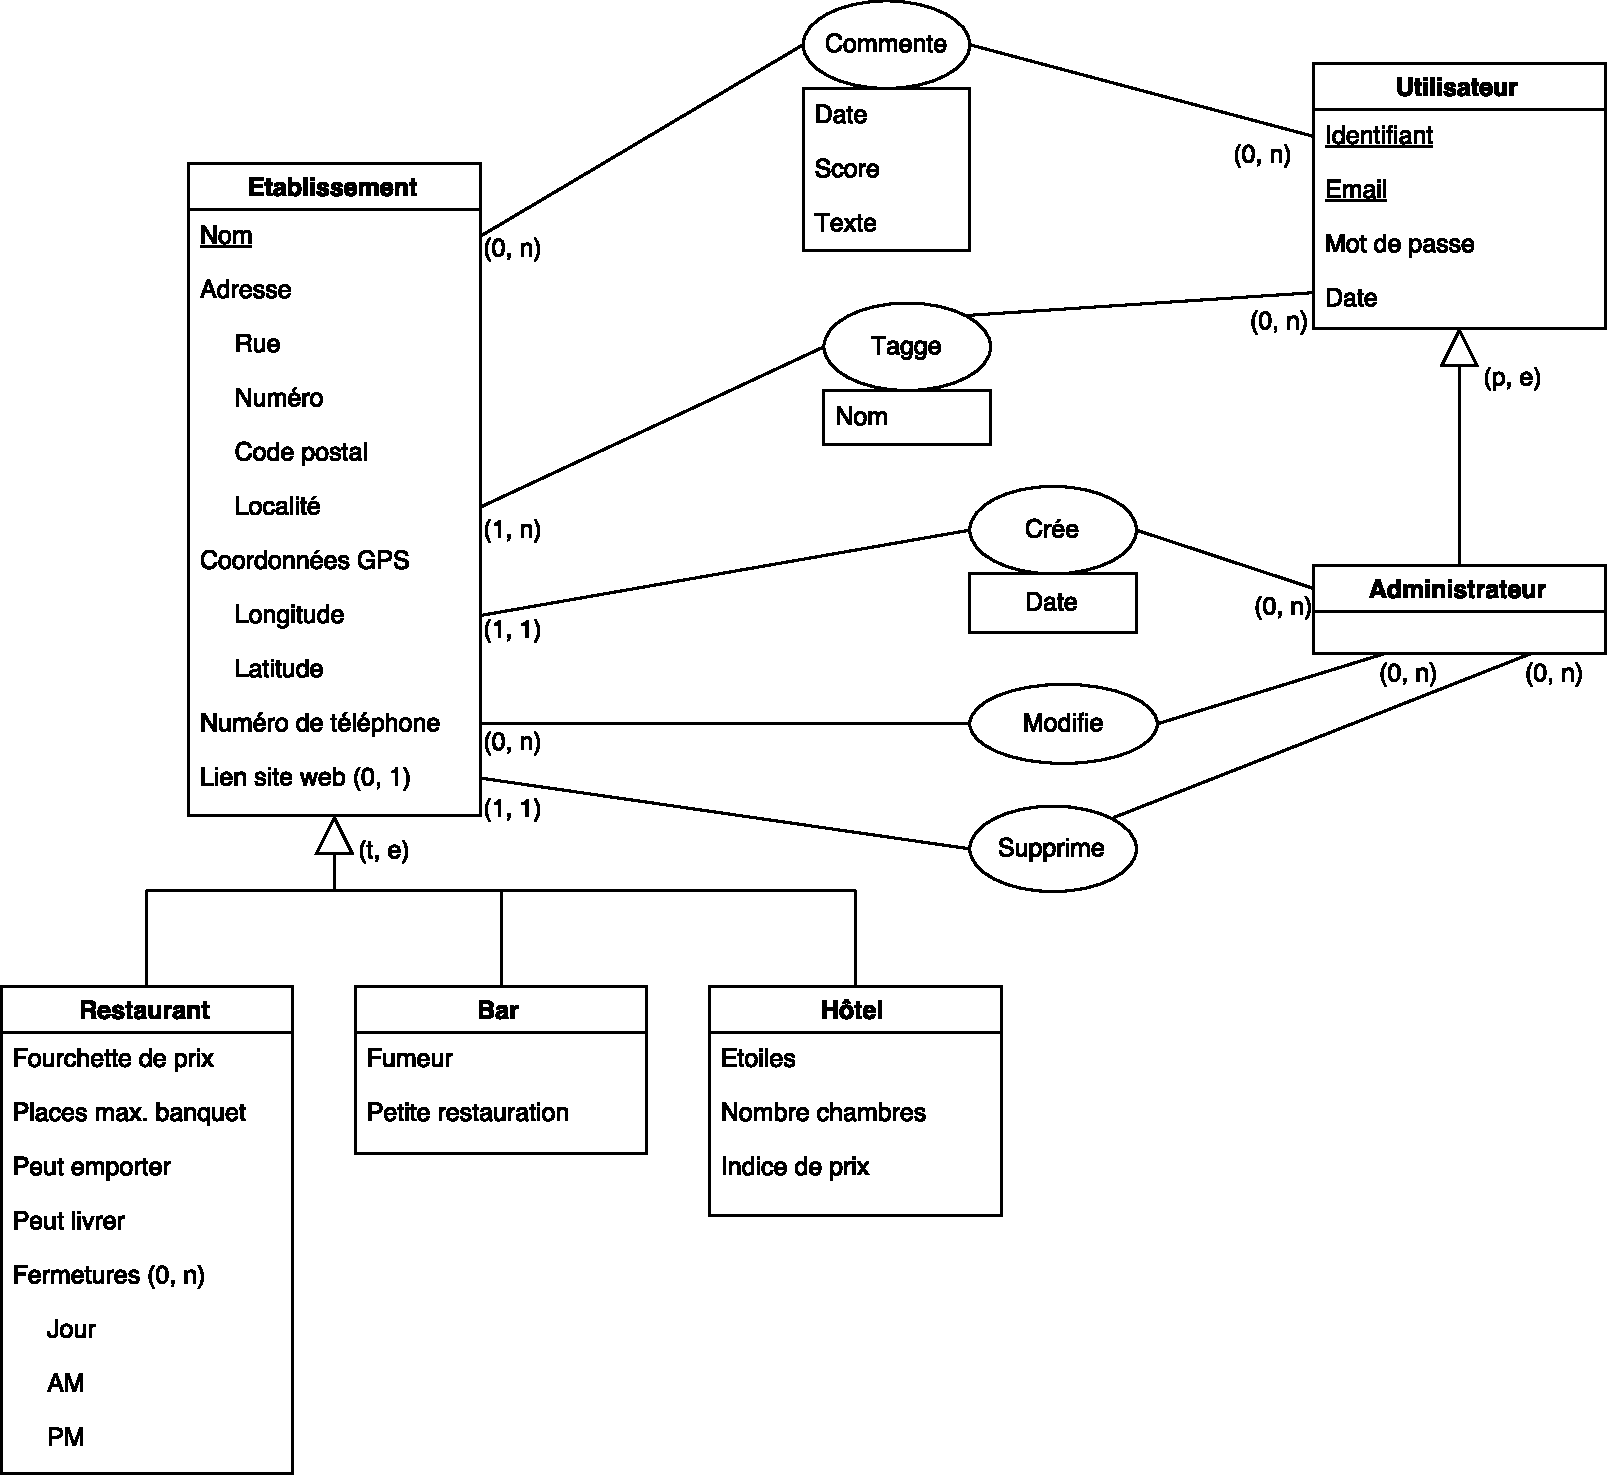
\includegraphics[scale=0.6]{horecaEA}
\end{center}

\section*{Contraintes d'intégrité}

\begin{itemize}
	\item[$\bullet$] L'adresse doit se trouver dans Bruxelles (même chose pour les coordonnées GPS).
	\item[$\bullet$] La date d'enregistrement d'un utilisateur précède la date de ses commentaires. 
	\item[$\bullet$] La date d'enregistrement d'un utilisateur précède la date de création de ses établissements.
	\item[$\bullet$] La date de création d'un établissement précède la date de ses commentaires.
	\item[$\bullet$] Le score dont est composé un commentaire est compris entre 0 et 5.
	\item[$\bullet$] Un utilisateur ne peut pas commenter un même établissement 2 fois le même jour.
	\item[$\bullet$] Un utilisateur peut tagger un établissement avec un nom de tag inexistant (il le crée) ou tagger avec un nom de tag existant (il le sélectionne). 
	\item[$\bullet$] Un utilisateur ne peut pas tagger un établissement 2 fois avec le même tag.
	\item[$\bullet$] Un hôtel a entre 0 et 5 étoiles.
\end{itemize}
\subsection*{Remarques}
\begin{itemize}
	\item[$\bullet$] Etant donné que les fermetures concernent chacune un jour de la semaine en renseignant sur la fermeture pour chaque demi-journée (AM/PM), un Restaurant ne peut avoir plus de 7 fermetures. 
\end{itemize}

\section*{Modèle relationnel}
\noindent
Utilisateur(\underline{Identifiant}, \underline{Email}, MotDePasse, Date, EstAdmin)\\
Etablissement(\underline{Nom}, AdresseRue, AdresseNuméro, AdresseCodePostal, AdresseLocalité, CoordonéesGPSLongitude, CoordonéesGPSLatitude, Numéro de téléphonne, \textit{LienSiteWeb})\\
Restaurant(\underline{Nom}, FouchettePrix, PlacesMaxBanquet, PeutEmporter, PeutLivrer)
\begin{itemize}
	\item[$\bullet$] Nom référence Etablissement.Nom
\end{itemize}
RestaurantFermetures(\underline{Nom, FermeturesJour, FermeturesAM, FermeturesPM})
\begin{itemize}
	\item[$\bullet$] Nom référence Etablissement.Nom
\end{itemize}
Bar(\underline{Nom}, Fumeur, PetiteRestauration)
\begin{itemize}
	\item[$\bullet$] Nom référence Etablissement.Nom
\end{itemize}
Hôtel(\underline{Nom}, Etoiles, NombreChambres, IndicePrix)
\begin{itemize}
	\item[$\bullet$] Nom référence Etablissement.Nom
\end{itemize}
Commente(\underline{Utilisateur, Etablissement}, Date, Score, Texte)
\begin{itemize}
	\item[$\bullet$] Utilisateur référence Utilisateur.Identifiant
	\item[$\bullet$] Nom référence Etablissement.Nom
\end{itemize}
Tagge(\underline{Utilisateur, Etablissement}, Nom)
\begin{itemize}
	\item[$\bullet$] Utilisateur référence Utilisateur.Identifiant
	\item[$\bullet$] Etablissement référence Etablissement.Nom
\end{itemize}
Crée(\underline{Créateur, Etablissement})
\begin{itemize}
	\item[$\bullet$] Créateur référence Utilisateur.Identifiant
	\item[$\bullet$] Nom référence Etablissement.Nom
\end{itemize}
Modifie(\underline{ModifiéPar, Etablissement})
\begin{itemize}
	\item[$\bullet$] ModifiéPar référence Utilisateur.Identifiant
	\item[$\bullet$] Nom référence Etablissement.Nom
\end{itemize}
Supprime({\underline{SuppriméPar}, NomEtablissement})
\begin{itemize}
	\item[$\bullet$] SuppriméPar référence Utilisateur.Identifiant
\end{itemize}
\subsection*{Contraintes d'intégrité supplémentaires}
\begin{itemize}
	\item[$\bullet$] L'Utilisateur référencé via Utilisateur.Identifiant dans Modifie, Supprime et Crée doit avoir EstAdmin à vrai.
\end{itemize}


\subsection*{Remarques}
\begin{itemize}
	\item[$\bullet$] NomEtablissement dans Supprime ne référence pas Etablissement.Nom étant donné que l'Etablissement sera supprimé. On utilise donc le nom de l'Etablissement supprimé, pas une clé.
\end{itemize}

\end{document}